\section{Introduction}

\subsection{Physical requirements for autonomous reaction mechanism research}

Scientific validation of an organic reaction mechanism requires checking the molecular geometries, reaction pathways, and quantum-chemical results assigned to each species and elementary step. Normal termination of a geometry optimization (exit 0) records completion of the program. Identifying a stable intermediate requires frequency analysis to confirm a minimum. Assigning a first-order saddle to a reaction step requires IRC calculations that identify the species connected on both sides. An intrinsic reaction coordinate (IRC) that reaches an unintended dissociation product or stereoisomer also changes the mechanistic assignment of the associated energy calculation. These checks are particularly important when a study includes several elementary steps or competing stereochemical pathways.\citep{ref09,ref10}

Computational chemistry agents automate several parts of this work. El Agente Q \citep{ref01}, Aitomia \citep{ref02}, and Gráfico \citep{ref06} orchestrate quantum-chemical calculations and typed workflows. Estructural \citep{ref04} and ARCHE \citep{ref05} provide tools for molecular fragment editing, atom mapping, and transition-state geometry preparation; Quntur \citep{ref03} addresses reaction kinetics and transition-state research. Extending these capabilities to autonomous mechanism exploration requires reliable geometric operations and physical interpretation of the species and pathways obtained.

Aligning stereochemical orientations, assembling reactant fragments, and preparing pathway endpoints require three-dimensional geometric reasoning. Language models can make errors when they infer spatial relationships or directly manipulate Cartesian coordinates. Quntur \citep{ref03}, for example, reports the need for human assistance with endpoint alignment in complex pathway and transition-state preparation. In Cloudra, an agent can ask the program to rotate the atoms on one side of a bond, measure the resulting dihedral angle, and compare the new geometry with another transition-state guess.

A proposed intermediate must optimize to a minimum. A candidate transition state must be a first-order saddle whose paths lead to the intended reactant and product. If an IRC reaches another product or stereoisomer, the saddle belongs to a different reaction from the one initially proposed. An autonomous system must use these results to reassign the step or search for another saddle.

\subsection{Cloudra: autonomous mechanism exploration through chemical objects}

We introduce Cloudra, a multi-agent system for exploring reaction mechanisms involving small organic molecules. Language models propose candidate pathways, choose calculations, and revise hypotheses from the returned structures and energies. The software maps atoms, moves molecular fragments, and runs geometry optimizations, frequency calculations, and IRCs. The results identify minima and saddle points and determine which species each saddle connects.

Figure~\ref{fig:01} summarizes a structured literature sample of 85 chemical AI agent systems: 39 concern materials or surfaces, 23 concern finite molecules or complexes, 12 concern soft matter or biomolecules, and 11 cover multiple categories of objects. Figures~\ref{fig:02} and \ref{fig:03} show the documented tasks in the finite-molecule/complex category and compare Cloudra's capabilities with those of the existing systems. The accompanying literature materials contain the complete matrix and the sources for each entry.

\begin{figure}[tbp]
\centering
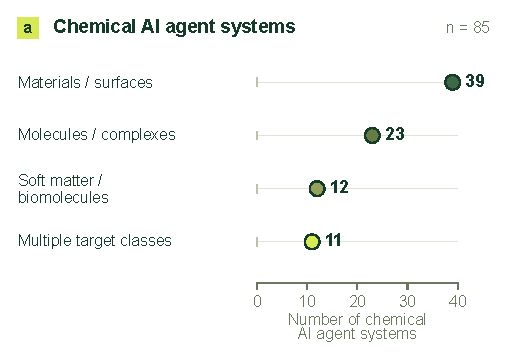
\includegraphics[width=\linewidth]{figures/fig01.pdf}
\caption{Physical targets in a structured literature sample of 85 chemical AI agent systems: 39 materials/surface, 23 finite-molecule/complex, 12 soft-matter/biomolecular, and 11 cross-class systems.}
\label{fig:01}
\end{figure}

Following intelligent restraint, Cloudra assigns coordinate calculations to deterministic routines. MCS matching selects molecular fragments; atom mapping matches reactant and product atoms and identifies atom pairs whose bonds change. The program measures bond lengths, bond angles, dihedral angles, and stereochemistry, and rotates or translates selected atoms to prepare candidate structures.

\begin{figure}[tbp]
\centering
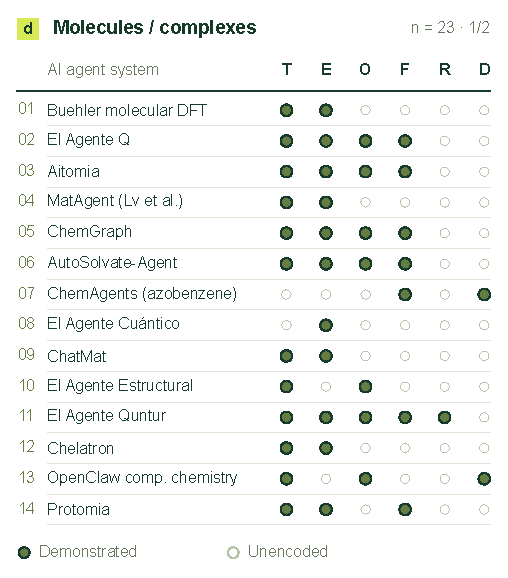
\includegraphics[width=\linewidth]{figures/fig02.pdf}
\caption{Documented tasks in the finite-molecule/complex class (panel 1 of 2; 23 chemical AI agent systems in total). T: structure construction/editing; E: static energy/properties; O: geometry optimization; F: vibrations/thermochemistry; R: explicit pathways/TS; D: molecular/quantum dynamics. Filled cells denote positive evidence; blanks leave capability coverage unspecified.}
\label{fig:02}
\end{figure}

The Delivery DAG represents chemical species as nodes and elementary reaction steps as edges. Nodes link to optimized geometries, energies, and frequencies; edges link to transition states and their IRC paths. A transition state must have exactly one imaginary frequency. The program checks that its frequency calculation and both IRC directions refer to the same saddle, and that optimizations from the IRC terminal frames reach the declared reactant and product species. The Supervisor reviews the resulting mechanism against the task and identifies calculations still needed and steps requiring further investigation.

\begin{figure}[tbp]
\centering
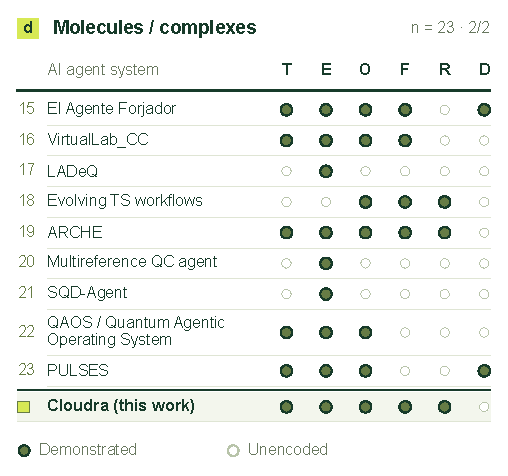
\includegraphics[width=\linewidth]{figures/fig03.pdf}
\caption{Chemical AI agent systems in the finite-molecule/complex class, continued (panel 2 of 2), using the codes in Figure~\ref{fig:02}. Cloudra (this work) is benchmarked at the bottom. Complete matrices for all 85 chemical AI agent systems and source-level qualifications accompany the draft.}
\label{fig:03}
\end{figure}

\subsection{Contributions}

Cloudra combines a DAG of species and elementary steps with algorithms for atom mapping, geometry construction, and stationary-point and pathway analysis. Atom mappings keep reactant and product atoms in a common order. Fragment operations generate candidate geometries, and frequency and IRC calculations determine which stationary points were found and which species they connect. The agents use these results to compare proposed steps, revise the mechanism, and select further calculations.

The geometric procedures include MCS-based fragment selection, graph traversal to select the atoms that move, and transition-state fragment assembly. They allow the agents to rotate selected groups, adjust fragment positions, measure the resulting structures, and prepare new guesses after an unsuccessful transition-state search.

We evaluate the framework's end-to-end mechanism-calculation capability using CloudraBench, which measures graph coverage, physical self-consistency, and task-defined target accuracy from native computational outputs. Its 50 tasks cover elementary and multistep reactions, stereochemistry, and the applicability limits of the allowed methods. The experiments comprise 48 independent runs with three repeats on four tasks and a completed study of 200 runs under four workflow configurations across all 50 tasks. Standard uses the same model backbone as the primary comparison; Record and Brief-errors examine evidence organization and diagnostic feedback.
